In this chapter we describe how we implement what we lay out in the Theory chapter.
\section{CamelsML}
Originally a fork of the code in \cite{lstm_second_paper} with a few modifications, 
the machine learning code of this thesis is now implemented to be a fully fledged 
Python package. As the original code it is forked from, it is released under the 
Apache 2.0 license and anyone is therefore free to modify and implement the code 
into their own experiments in the future.

We dub this package CamelsML (Camels Machine Learning).


See Appendix \ref{camelsml documentation} for documentation on how to use the python 
package.

\section{Model configuration}
\begin{figure}
\caption{Our full model configuration using an EA-LSTM \cite{lstm_second_paper}}.
\end{figure}
The models we apply in this thesis are all variants of the LSTM model described 
in \ref{LSTM Theory}.
\section{Data split}
With 671 basins in the CAMELS-GB dataset, we run into an issue with perhaps not 
having enough data. This is not a problem for the time series, as they have data 
over several years, but it is indeed a problem for the static features of which there 
are only one data point per basin. To improve our statistics we therefore use 
cross validation. All results in this thesis that compare models to each other 
are made from the same 5-fold cross validation split. The test set is separate 
from this and is only used to say something about our best performing model after 
we have analyzed the results.

\section{Training Algorithm}
\begin{figure}
\centering
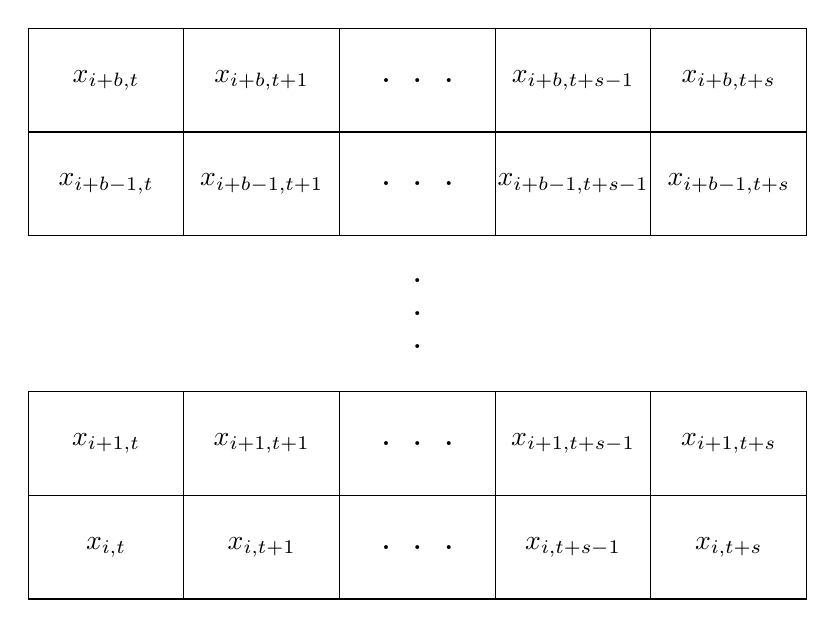
\begin{tikzpicture}[x=0.75pt,y=0.75pt,yscale=-1.25,xscale=1.25]
%uncomment if require: \path (0,300); %set diagram left start at 0, and has height of 300

%Shape: Rectangle [id:dp015989981921256002] 
\draw   (40,200) -- (340,200) -- (340,240) -- (40,240) -- cycle ;
%Shape: Rectangle [id:dp48971481940661865] 
\draw   (40,20) -- (340,20) -- (340,60) -- (40,60) -- cycle ;
%Straight Lines [id:da2960915083454566] 
\draw    (100,20) -- (100,60) ;
%Straight Lines [id:da243954626179525] 
\draw    (160,20) -- (160,60) ;
%Straight Lines [id:da4379878415202513] 
\draw    (220,20) -- (220,60) ;
%Straight Lines [id:da23623272729690736] 
\draw    (280,20) -- (280,60) ;
%Straight Lines [id:da34522789326312586] 
\draw    (100,200) -- (100,240) ;
%Straight Lines [id:da016177459682585327] 
\draw    (220,200) -- (220,240) ;
%Straight Lines [id:da5727133385469978] 
\draw    (280,200) -- (280,240) ;
%Straight Lines [id:da29038977274992184] 
\draw    (160,200) -- (160,240) ;






%Shape: Rectangle [id:dp015989981921256002] 
\draw   (40,160) -- (340,160) -- (340,200) -- (40,200) -- cycle ;
%Shape: Rectangle [id:dp48971481940661865] 
\draw   (40,60) -- (340,60) -- (340,100) -- (40,100) -- cycle ;

%Straight Lines [id:da2960915083454566] 
\draw    (100,60) -- (100,100) ;
%Straight Lines [id:da243954626179525] 
\draw    (160,60) -- (160,100) ;
%Straight Lines [id:da4379878415202513] 
\draw    (220,60) -- (220,100) ;
%Straight Lines [id:da23623272729690736] 
\draw    (280,60) -- (280,100) ;
%Straight Lines [id:da34522789326312586] 
\draw    (100,160) -- (100,200) ;
%Straight Lines [id:da016177459682585327] 
\draw    (220,160) -- (220,200) ;
%Straight Lines [id:da5727133385469978] 
\draw    (280,160) -- (280,200) ;
%Straight Lines [id:da29038977274992184] 
\draw    (160,160) -- (160,200) ;


% Text Node
\draw (190,40) node [anchor=center][inner sep=0.75pt]   [align=left] {{\LARGE . . .}};
% Text Node
\draw (190,220) node [anchor=center][inner sep=0.75pt]   [align=left] {{\LARGE . . .}};
% Text Node
\draw (190,130) node [anchor=center][inner sep=0.75pt]   [align=left] {{\LARGE .}\\{\LARGE .}\\{\LARGE .}};
% Text Node
\draw (70,220) node [anchor=center][inner sep=0.75pt]   [align=left] {$\bm{x}_{i,t}$};
% Text Node
\draw (70,40) node [anchor=center][inner sep=0.75pt]   [align=left] {$\bm{x}_{i+b,t}$};
% Text Node
\draw (130,220) node [anchor=center][inner sep=0.75pt]   [align=left] {$\bm{x}_{i,t+1}$};
% Text Node
\draw (130,40) node [anchor=center][inner sep=0.75pt]   [align=left] {$\bm{x}_{i+b,t+1}$};
% Text Node
\draw (250,40) node [anchor=center][inner sep=0.75pt]   [align=left] {$\bm{x}_{i+b,t+s-1}$};
% Text Node
\draw (250,220) node [anchor=center][inner sep=0.75pt]   [align=left] {$\bm{x}_{i,t+s-1}$};
% Text Node
\draw (310,40) node [anchor=center][inner sep=0.75pt]   [align=left] {$\bm{x}_{i+b,t+s}$};
% Text Node
\draw (310,220) node [anchor=center][inner sep=0.75pt]   [align=left] {$\bm{x}_{i,t+s}$};



\draw (190,80) node [anchor=center][inner sep=0.75pt]   [align=left] {{\LARGE . . .}};
% Text Node
\draw (190,180) node [anchor=center][inner sep=0.75pt]   [align=left] {{\LARGE . . .}};

\draw (70,180) node [anchor=center][inner sep=0.75pt]   [align=left] {$\bm{x}_{i+1,t}$};
% Text Node
\draw (70,80) node [anchor=center][inner sep=0.75pt]   [align=left] {$\bm{x}_{i+b-1,t}$};
% Text Node
\draw (130,180) node [anchor=center][inner sep=0.75pt]   [align=left] {$\bm{x}_{i+1,t+1}$};
% Text Node
\draw (130,80) node [anchor=center][inner sep=0.75pt]   [align=left] {$\bm{x}_{i+b-1,t+1}$};


% Text Node
\draw (250,80) node [anchor=center][inner sep=0.75pt]   [align=left] {$\bm{x}_{i+b-1,t+s-1}$};
% Text Node
\draw (250,180) node [anchor=center][inner sep=0.75pt]   [align=left] {$\bm{x}_{i+1,t+s-1}$};
% Text Node
\draw (310,80) node [anchor=center][inner sep=0.75pt]   [align=left] {$\bm{x}_{i+b-1,t+s}$};
% Text Node
\draw (310,180) node [anchor=center][inner sep=0.75pt]   [align=left] {$\bm{x}_{i+1,t+s}$};
\end{tikzpicture}

\caption{A minibatch. $\bm{x}_{i,t}$ represents the input parameters $\bm{x}$ at time step $t$ for time series $t \in [0, b]$ where $b$ is the batch size.}
\label{minibatch}
\end{figure}
Our training algorithm can be described as this:
\begin{enumerate}
    \item Split the basins in the training set into 5 parts. Repeat this 5 times, each time using 4/5 parts for training and 1/5 for validation.\begin{enumerate}
        \item Initialize LSTM model with random weights and zero biases, except for the bias of the forget gate $\bm{b}_f$ which is initialized as 5 to make the initial model either forget or remember idk \citationneeded
        \item Split each training basin's time series into len(time series) / sequence length parts, feeding batch size of these small parts into the model in parallel. 
        \item After running through these, update the parameters using ADAM.
        \item After an epoch, evaluate on the evaluation set. If early stopping is enabled, check whether or not to stop training.
    \end{enumerate}
\end{enumerate}
Evaluating our model is done using the Nash–Sutcliffe model efficiency coefficient (NSE). \cite{NSE}
This metric is similar to the $R^2$ score, but it is specialized for usage 
on hydrological time series.
It is defined as 
\begin{equation}
    \text{NSE} = 1 - \frac{\sum_{t=0}^T\left( y^t - \hat{y}^t\right)}{\sum_{t=0}^T\left(y^t - \bar{\hat{y}}\right)} \label{NSE}
\end{equation}
As we employ cross validation, what we actually end up with is 5 different models 
for each training run. These models do not necessarily converge to the same parameters 
as each other, making them potentially quite different from one another. To test the 
actual performance of a model (not just relative to other model configurations) we 
therefore need to train a new model with the same configuration (using the same features, 
hyperparameters, etc.) on the entire, undivided training set and test that model 
on the test set. This test result cannot be used to determine relative performance 
between different model configurations, but it can give an indication of the actual, 
real-world performance. "Absolute performance" versus "relative performance".

\section{Hardware}
